\documentclass[a4paper]{article}
\usepackage[UTF8]{ctex}
\usepackage[a4paper,margin=1in]{geometry}
\usepackage{graphicx}
\usepackage{float}
\usepackage{listings}
\usepackage{booktabs}
\usepackage{hyperref}
\usepackage{fancyhdr}
\usepackage{lastpage}
\usepackage{color}
\usepackage{xcolor}
\usepackage{indentfirst}        % 首段缩进
\setlength{\parindent}{2em}     % 缩进2字符
\usepackage{zhnumber}           % 中文编号
\usepackage[dvipsnames]{xcolor}
\usepackage{amsmath}

% ===== 个人信息与实验信息配置 =====
\newcommand{\projname}{议程管理系统Agenda}
\newcommand{\reporttitle}{实验2-测试报告}
\newcommand{\stuno}{23336179}
\newcommand{\authorname}{马福泉}
\newcommand{\major}{计算机科学与技术}
\newcommand{\adviser}{李文军}
\newcommand{\startdate}{2026年3月}
\newcommand{\labenddate}{2026年4月}
\newcommand{\labroom}{B201}

% ===== 页眉页脚设置 =====
\pagestyle{fancy} 
\fancyhf{}      
\fancyhead[L]{\kaishu \projname}      
\fancyhead[C]{\kaishu \reporttitle}    
\fancyhead[R]{\kaishu \authorname} 
\fancyfoot[C]{第 \thepage 页，共 \pageref{LastPage} 页} 
\renewcommand{\headrulewidth}{0.4pt}
\renewcommand{\footrulewidth}{0pt}

% ===== 代码高亮配置 (适应 Java) =====
\definecolor{NavyBlue}{RGB}{0,0,128}
\lstset{
    language=Java,
    basicstyle=\ttfamily\small,
    commentstyle=\color{gray}\itshape,
    keywordstyle=\color{blue}\bfseries,
    stringstyle=\color{red},
    breaklines=true,
    frame=single,
    numbers=left,
    numberstyle=\tiny\color{gray},
    tabsize=4,
    showstringspaces=false,
    captionpos=b,
    escapeinside={\%}{\%}
}

\begin{document}

% ==================== 封面 ====================
\begin{titlepage}
    \centering
    
    % 若没有校徽图片，可将下面这行注释掉
    
\includegraphics[width=10cm]{img/SYSULogo.png}

    \vspace{1em}
    {\Large \kaishu \projname \par}
    \vspace{3em}

    {\fontsize{36pt}{40pt}\kaishu \selectfont \boldmath \reporttitle\par}
    \vspace{2em}
    \vspace*{\fill}

    \begin{center}
    {\Large
    \makebox[5em][s]{学号}:\underline{\makebox[15em][c]{\kaishu \stuno}}\\[1em]
    \makebox[5em][s]{姓名}:\underline{\makebox[15em][c]{\kaishu \authorname}}\\[1em]
    \makebox[5em][s]{专业}:\underline{\makebox[15em][c]{\kaishu \major}}\\[1em]
    \makebox[5em][s]{指导教师}:\underline{\makebox[15em][c]{\kaishu \adviser}}\\[1em]
    \makebox[5em][s]{起始日期}:\underline{\makebox[15em][c]{\kaishu \startdate}}\\[1em]
    \makebox[5em][s]{结束日期}:\underline{\makebox[15em][c]{\kaishu \labenddate}}\\[1em]
    \makebox[5em][s]{实验地点}:\underline{\makebox[15em][c]{\kaishu \labroom}}
    }
    \end{center}

    \vspace*{\fill}
\end{titlepage}

% ==================== 目录 ====================
\tableofcontents
\newpage

% ==================== 正文 ====================

\section{系统启动与帮助菜单}

系统通过 \texttt{agenda.bat} 批处理脚本成功启动，如图~\ref{fig:terminal} 所示。启动后，系统正确显示了命令行提示符 \texttt{\$}，并打印了友好的欢迎界面。同时，系统完整列出了所有可用命令及其简要说明，包括 \texttt{register}（用户注册）、\texttt{add}（添加会议）、\texttt{query}（查询会议）、\texttt{delete}（删除会议）、\texttt{clear}（清除会议）、\texttt{batch}（批处理执行）以及 \texttt{quit}（退出系统）共七条核心命令。该设计完全符合实验指导书中关于"接口约定"的规范要求，用户可通过输入 \texttt{help} 命令随时查看帮助信息，体现了良好的人机交互设计。

\begin{figure}[H]
    \centering
    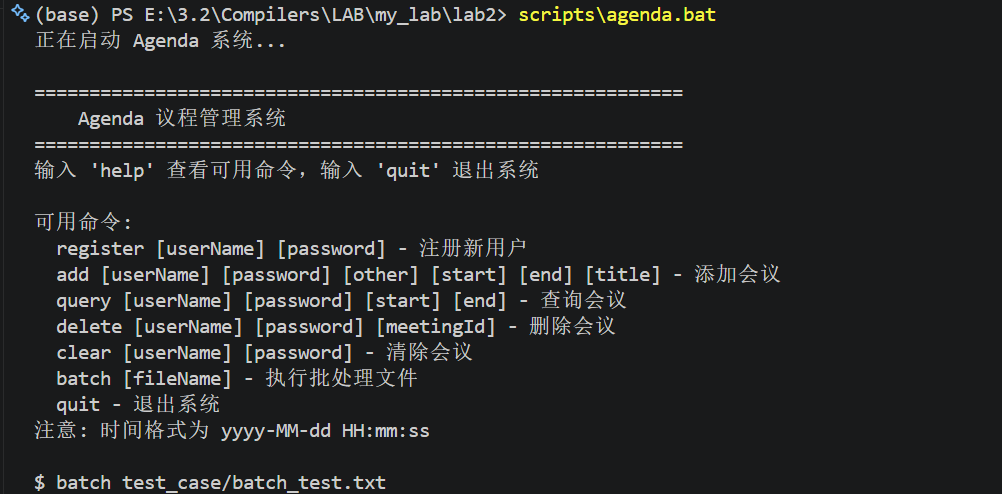
\includegraphics[width=0.9\textwidth]{img/terminal.png}
    \caption{系统启动界面与帮助菜单}
    \label{fig:terminal}
\end{figure}

\section{正常业务流程测试 (Happy Path)}

图~\ref{fig:1} 展示了系统在正常业务流程下的完整运行情况，验证了核心功能的正确性。

\textbf{（1）用户注册功能}：系统成功处理了用户注册请求，用户名和密码被正确存储，注册成功后返回明确的提示信息。

\textbf{（2）会议添加功能}：系统成功添加了多个会议。值得注意的是，截图展示了相邻时间段会议的无缝接续处理——当一个会议在 14:00 结束时，用户可以立即安排另一个从 14:00 开始的会议，系统正确识别这种边界情况为合法操作，体现了时间冲突检测算法的精确性。

\textbf{（3）会议查询功能}：\texttt{query} 命令的输出排版清晰，采用 \texttt{|} 分隔符对各字段进行格式化展示。更为关键的是，查询结果同时包含了该用户作为\textbf{发起人}（sponsor）和作为\textbf{被预约人}（scheduledUser）的会议记录。这一设计完美契合实验指导书中特别强调的易错点要求——即查询应返回用户参与的所有会议，而非仅返回用户发起的会议。

\textbf{（4）删除与清除功能}：系统正确执行了 \texttt{delete} 命令删除指定会议，以及 \texttt{clear} 命令清除用户发起的所有会议，操作结果反馈明确。

\begin{figure}[H]
    \centering
    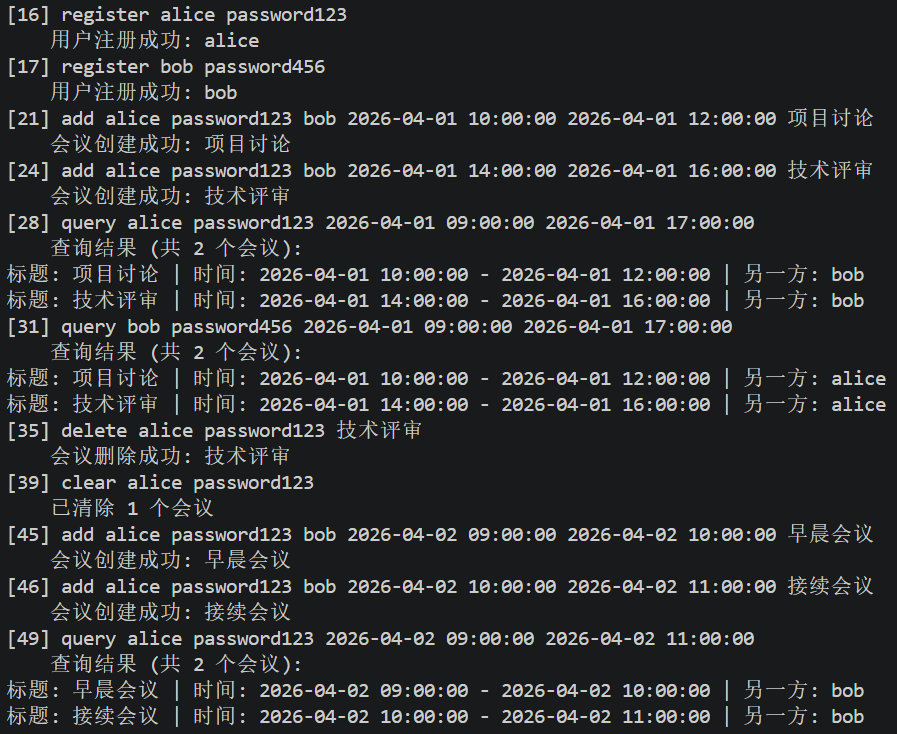
\includegraphics[width=0.9\textwidth]{img/1.png}
    \caption{正常业务流程测试}
    \label{fig:1}
\end{figure}

\section{核心业务异常与边界拦截}

图~\ref{fig:2} 集中展示了系统对各类异常情况的捕获与处理能力，充分体现了系统的健壮性设计。

\textbf{（1）用户认证异常}：系统成功拦截了重复用户名注册请求，抛出 \texttt{UserAlreadyExistsException} 异常；当用户密码输入错误时，系统返回认证失败提示，拒绝执行后续操作。

\textbf{（2）会议创建异常}：系统正确处理了"被预约用户不存在"的情况，以及"发起人与被预约人不能是同一人"的非法会议创建请求，分别抛出 \texttt{UserNotFoundException} 和 \texttt{SameUserException} 异常。

\textbf{（3）时间冲突检测（核心亮点）}：这是本系统最重要的健壮性特性。截图清晰展示了时间冲突检测的全面性：
\begin{itemize}
    \item 当发起人在请求的时间段内已有其他会议安排时，系统精准识别并提示"发起人时间冲突"；
    \item 当被预约人在请求的时间段内存在时间重叠的会议时，系统同样能够准确检测并提示"被预约人时间冲突"。
\end{itemize}

该功能基于德摩根定律推导的时间冲突判定算法实现：若两个时间段 $[s_1, e_1]$ 与 $[s_2, e_2]$ 满足 $s_1 < e_2 \land s_2 < e_1$，则存在重叠。系统对所有可能的冲突场景均给出了友好的中文错误提示，用户体验良好。

\begin{figure}[H]
    \centering
    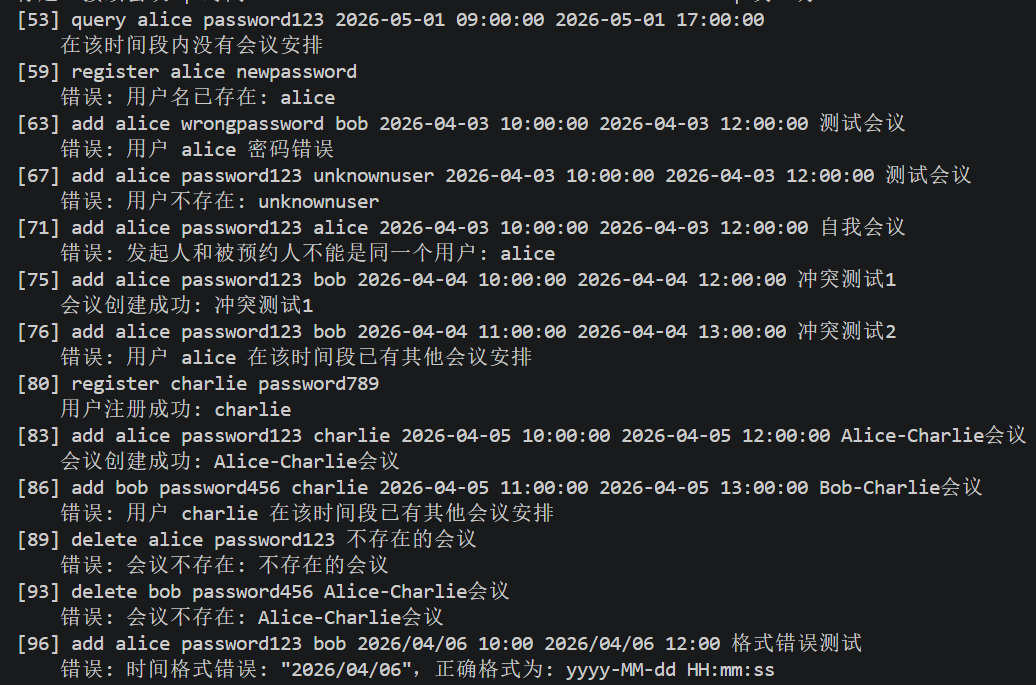
\includegraphics[width=0.9\textwidth]{img/2.png}
    \caption{核心业务异常与边界拦截测试}
    \label{fig:2}
\end{figure}

\section{命令健壮性与自动化回归测试}

\subsection{参数与命令健壮性}

图~\ref{fig:3} 展示了系统对非法输入的容错处理能力。当用户输入未知命令时，系统不会崩溃或抛出未处理的异常，而是友好地提示"未知命令"并列出可用命令。当用户输入参数不足时（如单独输入 \texttt{register} 而不提供用户名和密码），系统会捕获 \texttt{InvalidCommandException} 异常，并打印详细的用法说明（Usage），包括命令格式、参数要求以及时间格式规范。这种高容错设计确保了系统在面对各种异常输入时仍能稳定运行。

\begin{figure}[H]
    \centering
    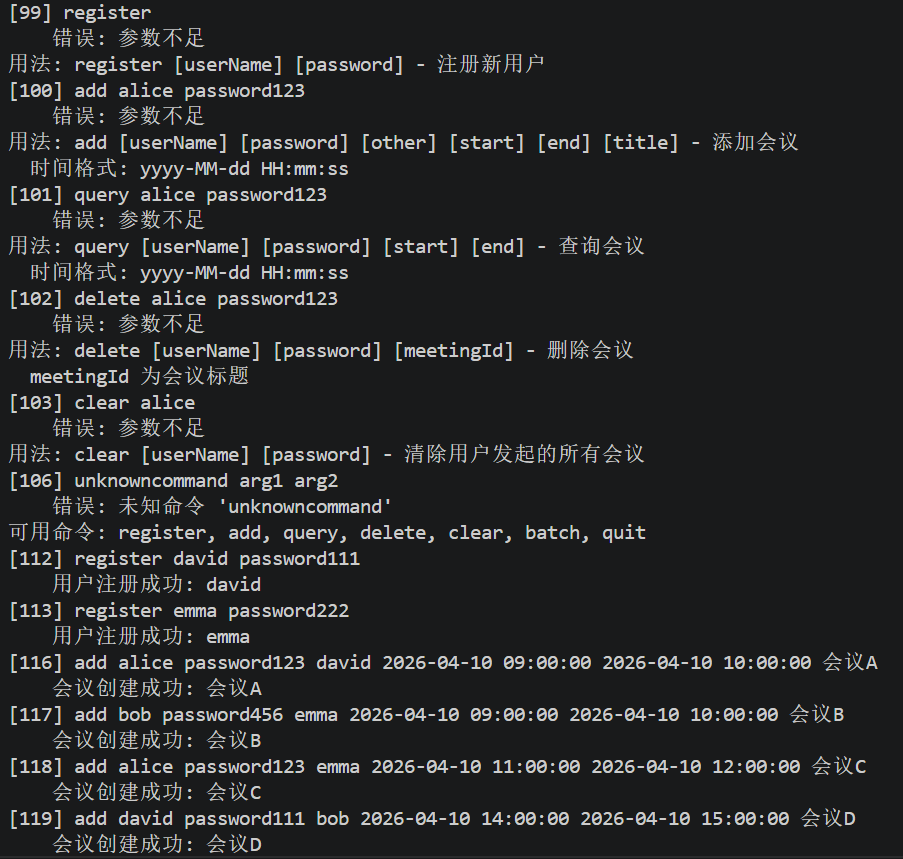
\includegraphics[width=0.9\textwidth]{img/3.png}
    \caption{命令健壮性测试}
    \label{fig:3}
\end{figure}

\subsection{自动化批处理支持}

图~\ref{fig:4} 展示了系统对批处理命令的支持情况。通过 \texttt{\$ batch [fileName]} 命令，用户可以执行预定义的测试脚本文件。系统在执行过程中会清晰地打印每条命令的行号标识（如 \texttt{[122]}），便于定位和调试。执行完毕后，系统自动统计并输出运行概况，如"批处理完成：成功 30 个，失败 15 个"，直观展示测试通过率。

这一设计极大地便利了系统的自动化回归测试（Regression Testing）。开发人员可以预先编写包含大量测试用例的脚本文件，通过批处理命令一次性执行，快速验证系统功能的正确性，显著提高了测试效率。

\begin{figure}[H]
    \centering
    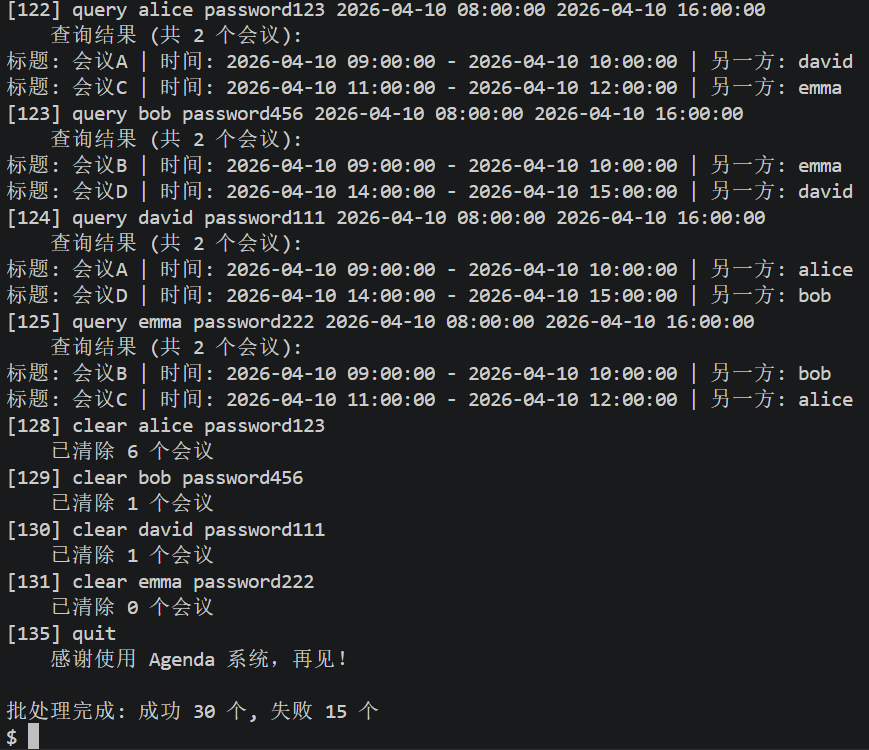
\includegraphics[width=0.9\textwidth]{img/4.png}
    \caption{自动化批处理测试}
    \label{fig:4}
\end{figure}

\end{document}